\documentclass[12pt, twoside]{article}
\usepackage[letterpaper, margin=1in, headsep=0.5in]{geometry}
\usepackage[english]{babel}
\usepackage[utf8]{inputenc}
\usepackage{amsmath}
\usepackage{amsfonts}
\usepackage{amssymb}
\usepackage{tikz}
\usetikzlibrary{quotes, angles}

\usepackage{pgfplots}
\pgfplotsset{width=9cm,compat=1.9}

\usepackage{venndiagram}
\usepackage{multicol}

\usepackage{fancyhdr}
\pagestyle{fancy}
\fancyhf{}
\renewcommand{\headrulewidth}{0pt} % disable the underline of the header
%\renewcommand{\baselinestretch}{1.5}

\fancyhead[LE]{\thepage}
\fancyhead[RO]{\thepage \\ Name: \hspace{3cm}}
\fancyhead[LO]{BECA / Dr. Huson / IB Math\\* 25 November 2019}


\begin{document}
\subsubsection*{2.19 Exam: Descriptive statistics}

\begin{enumerate}
  \subsubsection*{Write your answers on the exam in the space provided. Show work as required.}
  \item If you have not emailed me a copy of your exploration project paper, please explain here. Include why it is late, when you plan to email it to me, and what I can do to help you.  \vspace{6cm}
  
  \item The following box-and-whisker plot represents the examination scores of a group of students.\\
  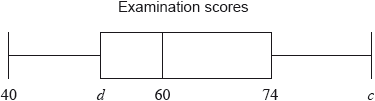
\includegraphics[width=9cm]{2-16exam-scores-box-plot.png}
  \begin{enumerate}
    \item Write down the median score. \hfill [1 marks]\\[1.5cm]
    The range of the scores is 54 marks, and the interquartile range is 21 marks.
    \item Find the value of
    \begin{enumerate}
      \item $c$; \hfill [2 marks] \vspace{2cm}
      \item $d$. \hfill [2 marks] \vspace{2cm}
    \end{enumerate}
  \end{enumerate}

  \newpage
  \item Given the following set of 15 data:
    \begin{center}
    3, 4, 4, 5, 5, 5, 6, 8, 9, 11, 11, 15, 15, 16, 17
  \end{center}
  \begin{enumerate}
    \item Write down the mode \hfill [1 marks] \vspace{1cm}
    \item Find the median. \hfill [1 marks] \vspace{1.5cm}
    \item Find the interquartile range. \hfill [2 marks] \vspace{3cm}
    \item Draw a box and whiskers plot of the data on the axis below. \hfill [2 marks] \vspace{1cm}
      \begin{center}
        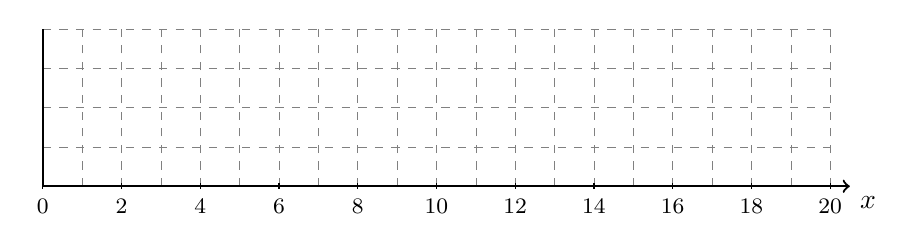
\begin{tikzpicture}[scale=.5]
          \draw [help lines, dashed] (0,0) grid (20,4);
          \draw [thick, ->] (0,0) -- (20.5,0) node [below right] {$x$};
          \foreach \x in {0,2,4,6,8,10, 12, 14, 16, 18, 20}
            \draw[shift={(\x,0)},color=black] (0pt,2pt) -- (0pt,-2pt) node[below] {\footnotesize $\x$};
          \draw [thick, -] (0,0)--(0,4);
        \end{tikzpicture}
      \end{center} \vspace{1cm}
      \item Find the mean. \hfill [2 marks]
    \end{enumerate}

\newpage

  \item There are 250 high school students at BECA ranging in age from 13 to 18 years old. The following table shows the frequencies of each age.
    \begin{center}
    \begin{tabular}{|l|r|r|r|r|r|r|}
      \hline
      Age (years) & 13 & 14 & 15 & 16 & 17 & 18\\ 
      \hline 
      Frequency & 27 & 53 & 60 & $k$ & 43 & 12\\ 
      \hline 
      \end{tabular}
    \end{center}

  \begin{enumerate}
    \item Calculate the value of $k$. \hfill [1 mark] \vspace{1.5cm}
    \item Write down the mode. \hfill [1 mark] \vspace{1.5cm}
    \item Find the value of the range. \hfill [1 marks] \vspace{1.5cm}
    \item Find the median. \hfill [1 marks] \vspace{1.5cm}
    \item Find the mean. \hfill [2 marks] \vspace{1.5cm}
    \item Find the standard deviation. \hfill [2 marks] \vspace{1.5cm}
    \item Four years later the same 250 people have moved on to college and career. Find the new values of the 
    \begin{enumerate}
      \item mean; \hfill [1 marks] \vspace{1.5cm}
      \item standard deviation. \hfill [1 marks]
    \end{enumerate}
  \end{enumerate}

\newpage
  \item The following diagram shows triangle $ABC$ (not drawn to scale).
  \begin{center}
    \begin{tikzpicture}[scale=1.4, rotate=-15]
      \draw [-, thick] (54:3) node[above right]{$C$}--
        (0,0) node[left]{$A$}--
        (4.5,0) node[right]{$B$}--cycle;
      \node at (0.3, 0.2)[right]{$56^\circ$};
      \node at (4, 0.2)[above left]{$46^\circ$};
      \node at (3.3, 1.7)[below]{$7$};
    \end{tikzpicture}
    \end{center} 
    $BC=7$, $C\hat{A}B=56^\circ$, and $A\hat{B}C=46^\circ$
    \begin{enumerate}
      \item Find the measure of $A\hat{C}B$. \hfill [1 mark1] \vspace{3cm}
      \item Find $AC$. \hfill [3 marks] \vspace{5cm}
      \item Find the area of triangle $ABC$. \hfill [3 marks] \vspace{5cm}
    \end{enumerate}
    
\newpage
  \item The histogram below shows the heart rate $x$ in beats per minute for 65 athletes after a fitness exercise.

    \begin{center}
      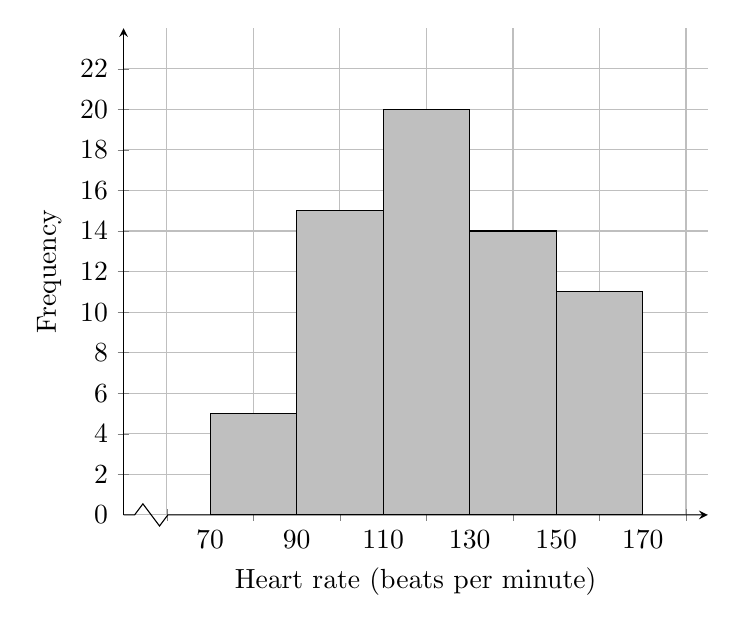
\begin{tikzpicture}
      \begin{axis}[
        xlabel=Heart rate (beats per minute),
        ylabel=Frequency,
        ybar interval=1,
        xmin=60, xmax=195,
        ymin=0, ymax=24,
        xtick={70,90,110,130,150,170,190},
        ytick={0,2,4,6,8,10,12,14,16,18,20,22},
        axis lines = left,
        ymajorgrids=true,
        axis x discontinuity=crunch,
      ]
      \addplot+ [color=black, fill=lightgray]
        coordinates {(80,5) (100,15)
          (120,20) (140,14) 
          (160,11) 
          (180,3)}; %Last pair does not show
      \end{axis}
      \end{tikzpicture}
    \end{center}

    The following is the frequency table for the distribution of $x$. \\[0.25cm]
      \begin{tabular}{|l|c|c|c|c|c|}
        \hline
        HR ($x$) & $70 \leq x < 90$ & $90 \leq x < 110$ & $110 \leq x < 130$ & $130 \leq x < 150$ & $150 \leq x < 170$ \\ 
        \hline 
        Freq & 5 & $p$ & 20 & 14 & 11  \\ 
        \hline 
        \end{tabular}
      \begin{enumerate}
        \item Write down the value of $p$. \hfill [1 mark] \vspace{1cm}
        \item Write down the modal class. \hfill [2 marks] \vspace{1cm}
        \item An athlete is selected at random. Find the probability that the athlete has a heart rate of 130 beats per minute or greater. \hfill [2 marks] \vspace{1cm}
        \item Consider the class interval $70 \leq x < 90$.
        \begin{enumerate}
          \item Write down the interval width. \hfill [1 mark] \vspace{1cm}
          \item Write down the mid-interval value. \hfill [1 mark] 
        \end{enumerate}
        \item Hence find an estimate for the
        \begin{enumerate}
          \item mean; \hfill [2 marks] \vspace{1cm}
          \item standard deviation. \hfill [2 marks] 
        \end{enumerate}
      \end{enumerate}

    
\newpage
  \item The following diagram shows quadrilateral $ABCD$ (not drawn to scale).
  \begin{center}
    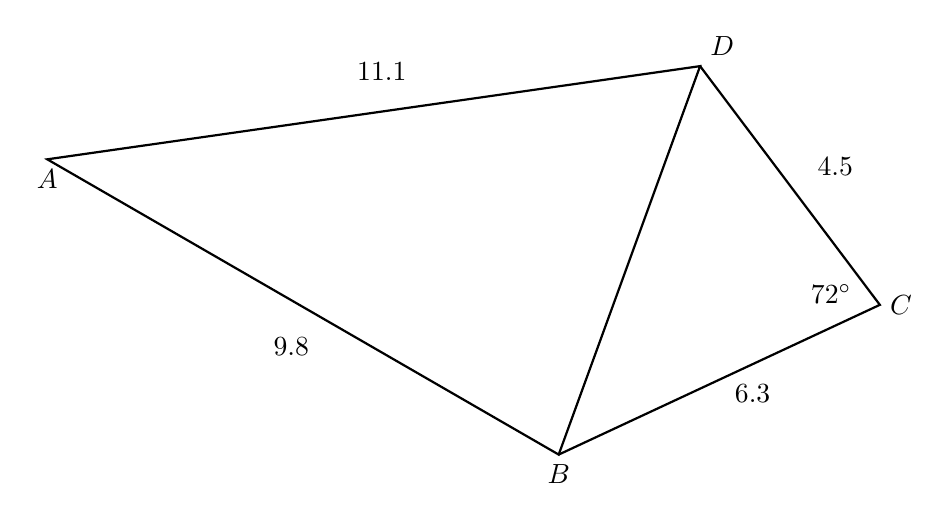
\begin{tikzpicture}[scale=1.5, rotate=-30]
      \draw [-, thick] (100:3.5) node[above right]{$D$}--
        (0,0) node[below]{$B$}--
        (-5,0) node[below]{$A$}--cycle;
      \draw [-, thick] (100:3.5) --
      (55:3) node[right]{$C$}--
      (0,0);             
      \node at (58:2.9)[left]{$72^\circ$};
      \node at (50:1.5)[right]{$6.3$};
      \node at (-2.5,-0.2)[below]{$9.8$};
      \node at (78:3.5)[below]{$4.5$};
      \node at (-3,2.2)[below]{$11.1$};
    \end{tikzpicture}
    \end{center} 
    $AB=9.8$, $BC=6.3$, $CD=4.5$, $AD=11.1$, and $B\hat{C}D=72^\circ$
    \begin{enumerate}
      \item Find $BD$. \hfill [3 marks] \vspace{6cm}
      \item Find $A\hat{B}D$. \hfill [3 marks]
    \end{enumerate}

\end{enumerate}
\end{document}

\item Consider the following frequency table.
\begin{center}
  \begin{tabular}{|c|c|}
    \hline
    $x$ & Frequency\\ 
    \hline 
    10 & 2 \\ 
    \hline 
    11 & 6 \\ 
    \hline 
    12 & 11 \\ 
    \hline 
    13 & 12 \\ 
    \hline 
    14 & 8 \\ 
    \hline 
    15 & 3 \\ 
    \hline 
    \end{tabular}
\end{center}

\begin{enumerate}
  \item Write down the mode \hfill [1 marks] \vspace{1cm}
  \item Find the value of the range. \hfill [2 marks] \vspace{1.5cm}
  \item Find the value of the mean. \hfill [2 marks] \vspace{1cm}
  \item Find the value of the standard deviation. \hfill [2 marks]
\end{enumerate}
\vspace{1cm}


\item The scores of 30 students taking an IB Paper 2 are shown in the frequency table below.
    
\begin{tabular}{|l|c|c|c|c|}
  \hline
  Mark ($x$) & $10 \leq x < 30$ & $30 \leq x < 50$ & $50 \leq x < 70$ & $70 \leq x < 90$\\ 
  \hline 
  Frequency & 8 & 12 & 7 & 3\\ 
  \hline 
  \end{tabular}

\begin{enumerate}
  \item Write down the modal class.  \hfill [1 mark]  \vspace{2cm}
  \item Estimate the mean score $\overline{x}$. \hfill [3 marks] \vspace{2cm}
  \item Estimate the standard deviation of the scores, $\sigma$.  \hfill [3 marks] \vspace{1cm}
\end{enumerate}